\documentclass[../thesis/thesis.tex]{subfiles}
\begin{document}
 \chapter{Orphans: Node Structure}

\section{Node Hardware}
 
\begin{figure}
\centering
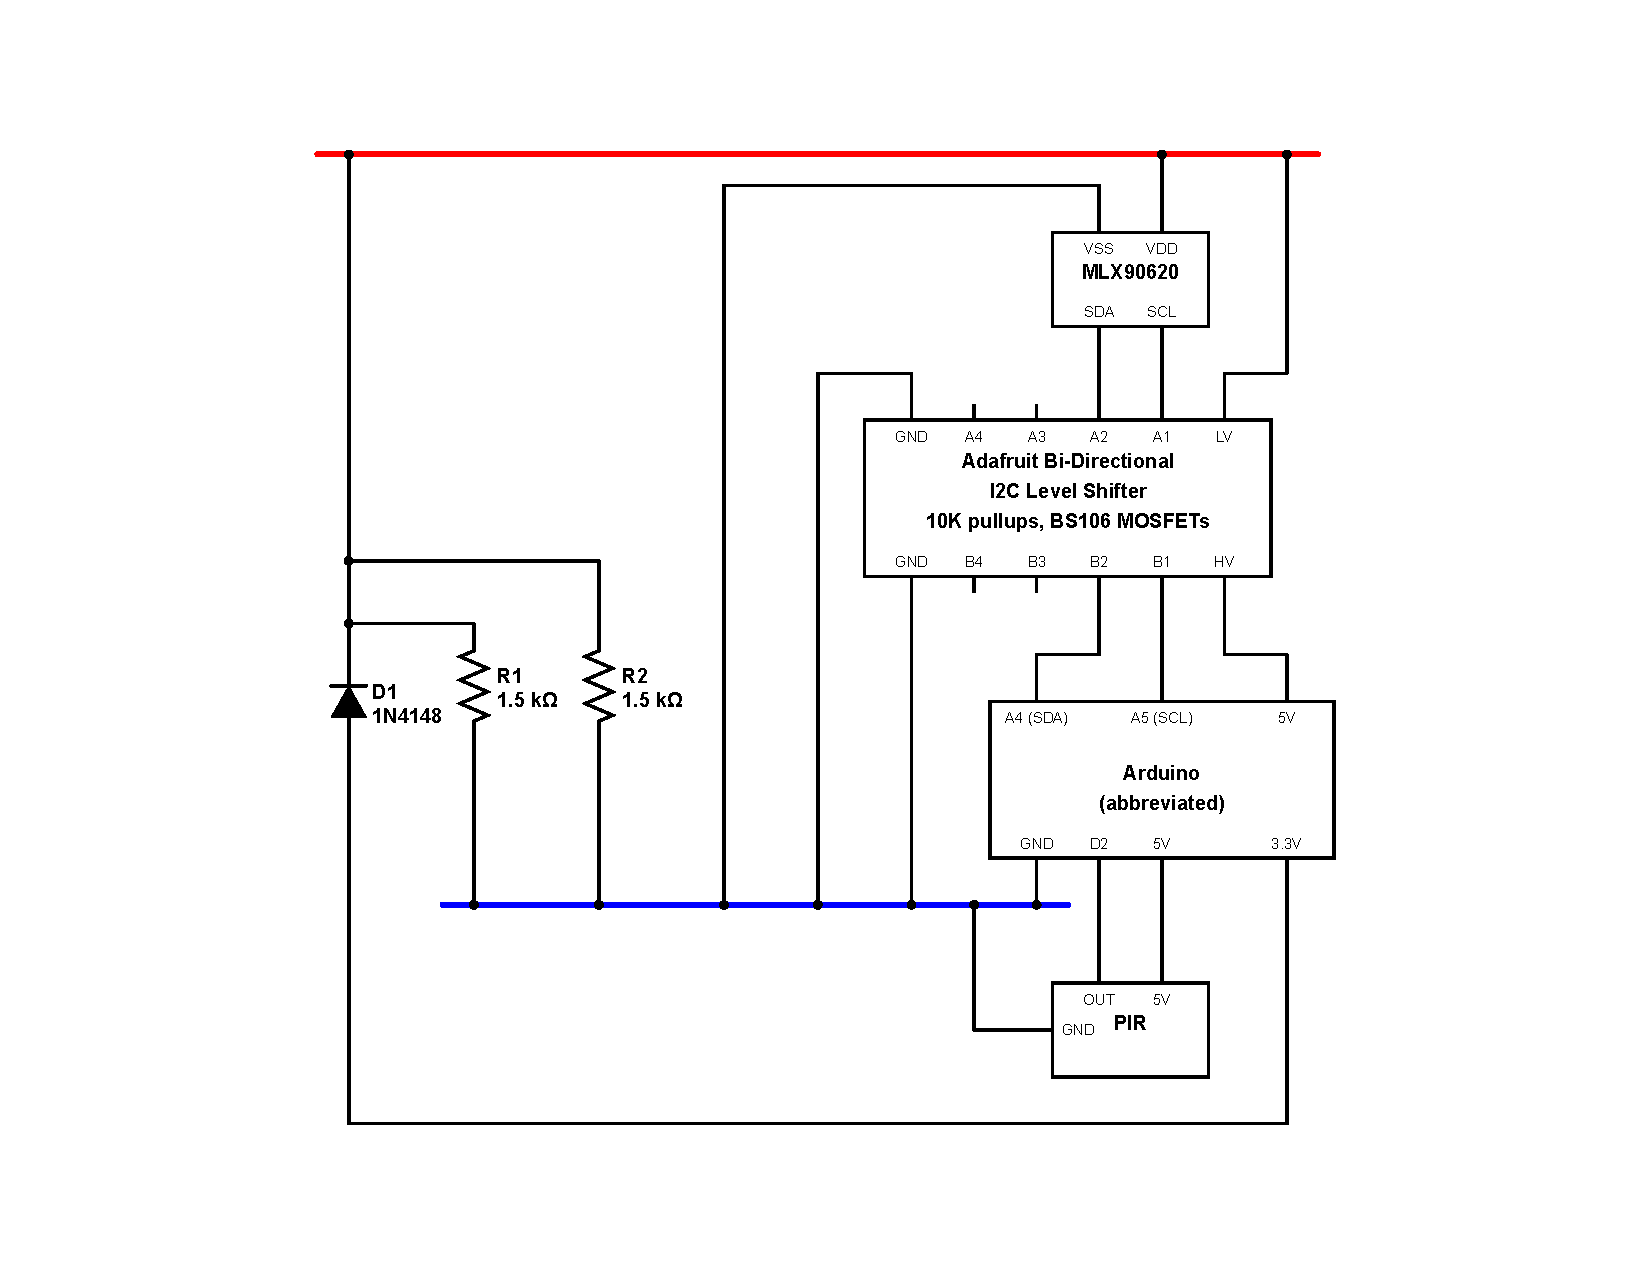
\includegraphics[width=\textwidth]{../diagrams/mlx-arduino.pdf}
\caption{MLX90620 and Arduino integration circuit}
\label{fig:circuits:node}
\end{figure}

Due to low cost and ease of use, the \ard platform was selected as the host for the low-level \iic interface for communication to the \mlx. Initially, this presented some challenges, as the \mlx recommends a power and communication voltage of 2.6V, while the \ard is only able to output 3.3V and 5V as power, and 5V as communication. Due to this, it was not possible to directly connect the \ard to the \mlx, and similarly due to the two-way nature of the \iic 2-wire communication protocol, it was also not possible to simply lower the \ard voltage using simple electrical techniques, as such techniques would interfere with two-way communication.

A solution was found in the form of a \iic level-shifter, the Adafruit ``4-channel I2C-safe Bi-directional Logic Level Converter'' \cite{AdafruitI2C}, which provided a cheap method to bi-directionally communicate between the two devices at their own preferred voltages. The layout of the circuit necessary to link the \ard and the \mlx using this converter can be seen in \Fref{fig:circuits:node}.

\section{Node Software}

To calculate the final temperature values that the \mlx offers, a complex initialisation and computational process must be followed, which is specified in the sensor's datasheet \cite{MLXDatasheet}. This process involves initialising the sensor with values attained from a separate on-board \iic EEPROM, then retrieving a variety of normalisation and adjustment values, along with the raw sensor data, to compute the final temperature result.

The basic algorithm to perform this normalisation was based upon code by users ``maxbot'', ``IIBaboomba'', ``nseidle'' and others on the Arduino Forums \cite{ArduinoForum} and was modified to operate with the newer \ard \iic libraries released since the authors' posts. In pursuit of the project's aims to create a more approachable thermal sensor, the code was also restructured and rewritten with more comments and named constants so that the code is more readily understood and easier to modify for other purposes.



\begin{figure}
 \centering
\begin{lstlisting}[style=arduino]
INIT 0
INFO START
DRIVER MLX90620
BUILD Feb  1 2015 00:00:00
IRHZ 1
INFO STOP
ACTIVE 33
\end{lstlisting}
\caption{Initialisation sequence}
\label{fig:code:initseq}
\end{figure}

\begin{figure}
 \centering
\begin{lstlisting}[style=arduino]
START 34
MOVEMENT 0
1.0  1.0  1.0  1.0  1.0  1.0  1.0  1.0  1.0  1.0  1.0  1.0  1.0  1.0  1.0  1.0
1.0  1.0  1.0  1.0  1.0  1.0  1.0  1.0  1.0  1.0  1.0  1.0  1.0  1.0  1.0  1.0
1.0  1.0  1.0  1.0  1.0  1.0  1.0  1.0  1.0  1.0  1.0  1.0  1.0  1.0  1.0  1.0
1.0  1.0  1.0  1.0  1.0  1.0  1.0  1.0  1.0  1.0  1.0  1.0  1.0  1.0  1.0  1.0
STOP 97
\end{lstlisting}
\caption{Thermal data packet}
\label{fig:code:packet}
\end{figure}

\begin{figure}
\centering
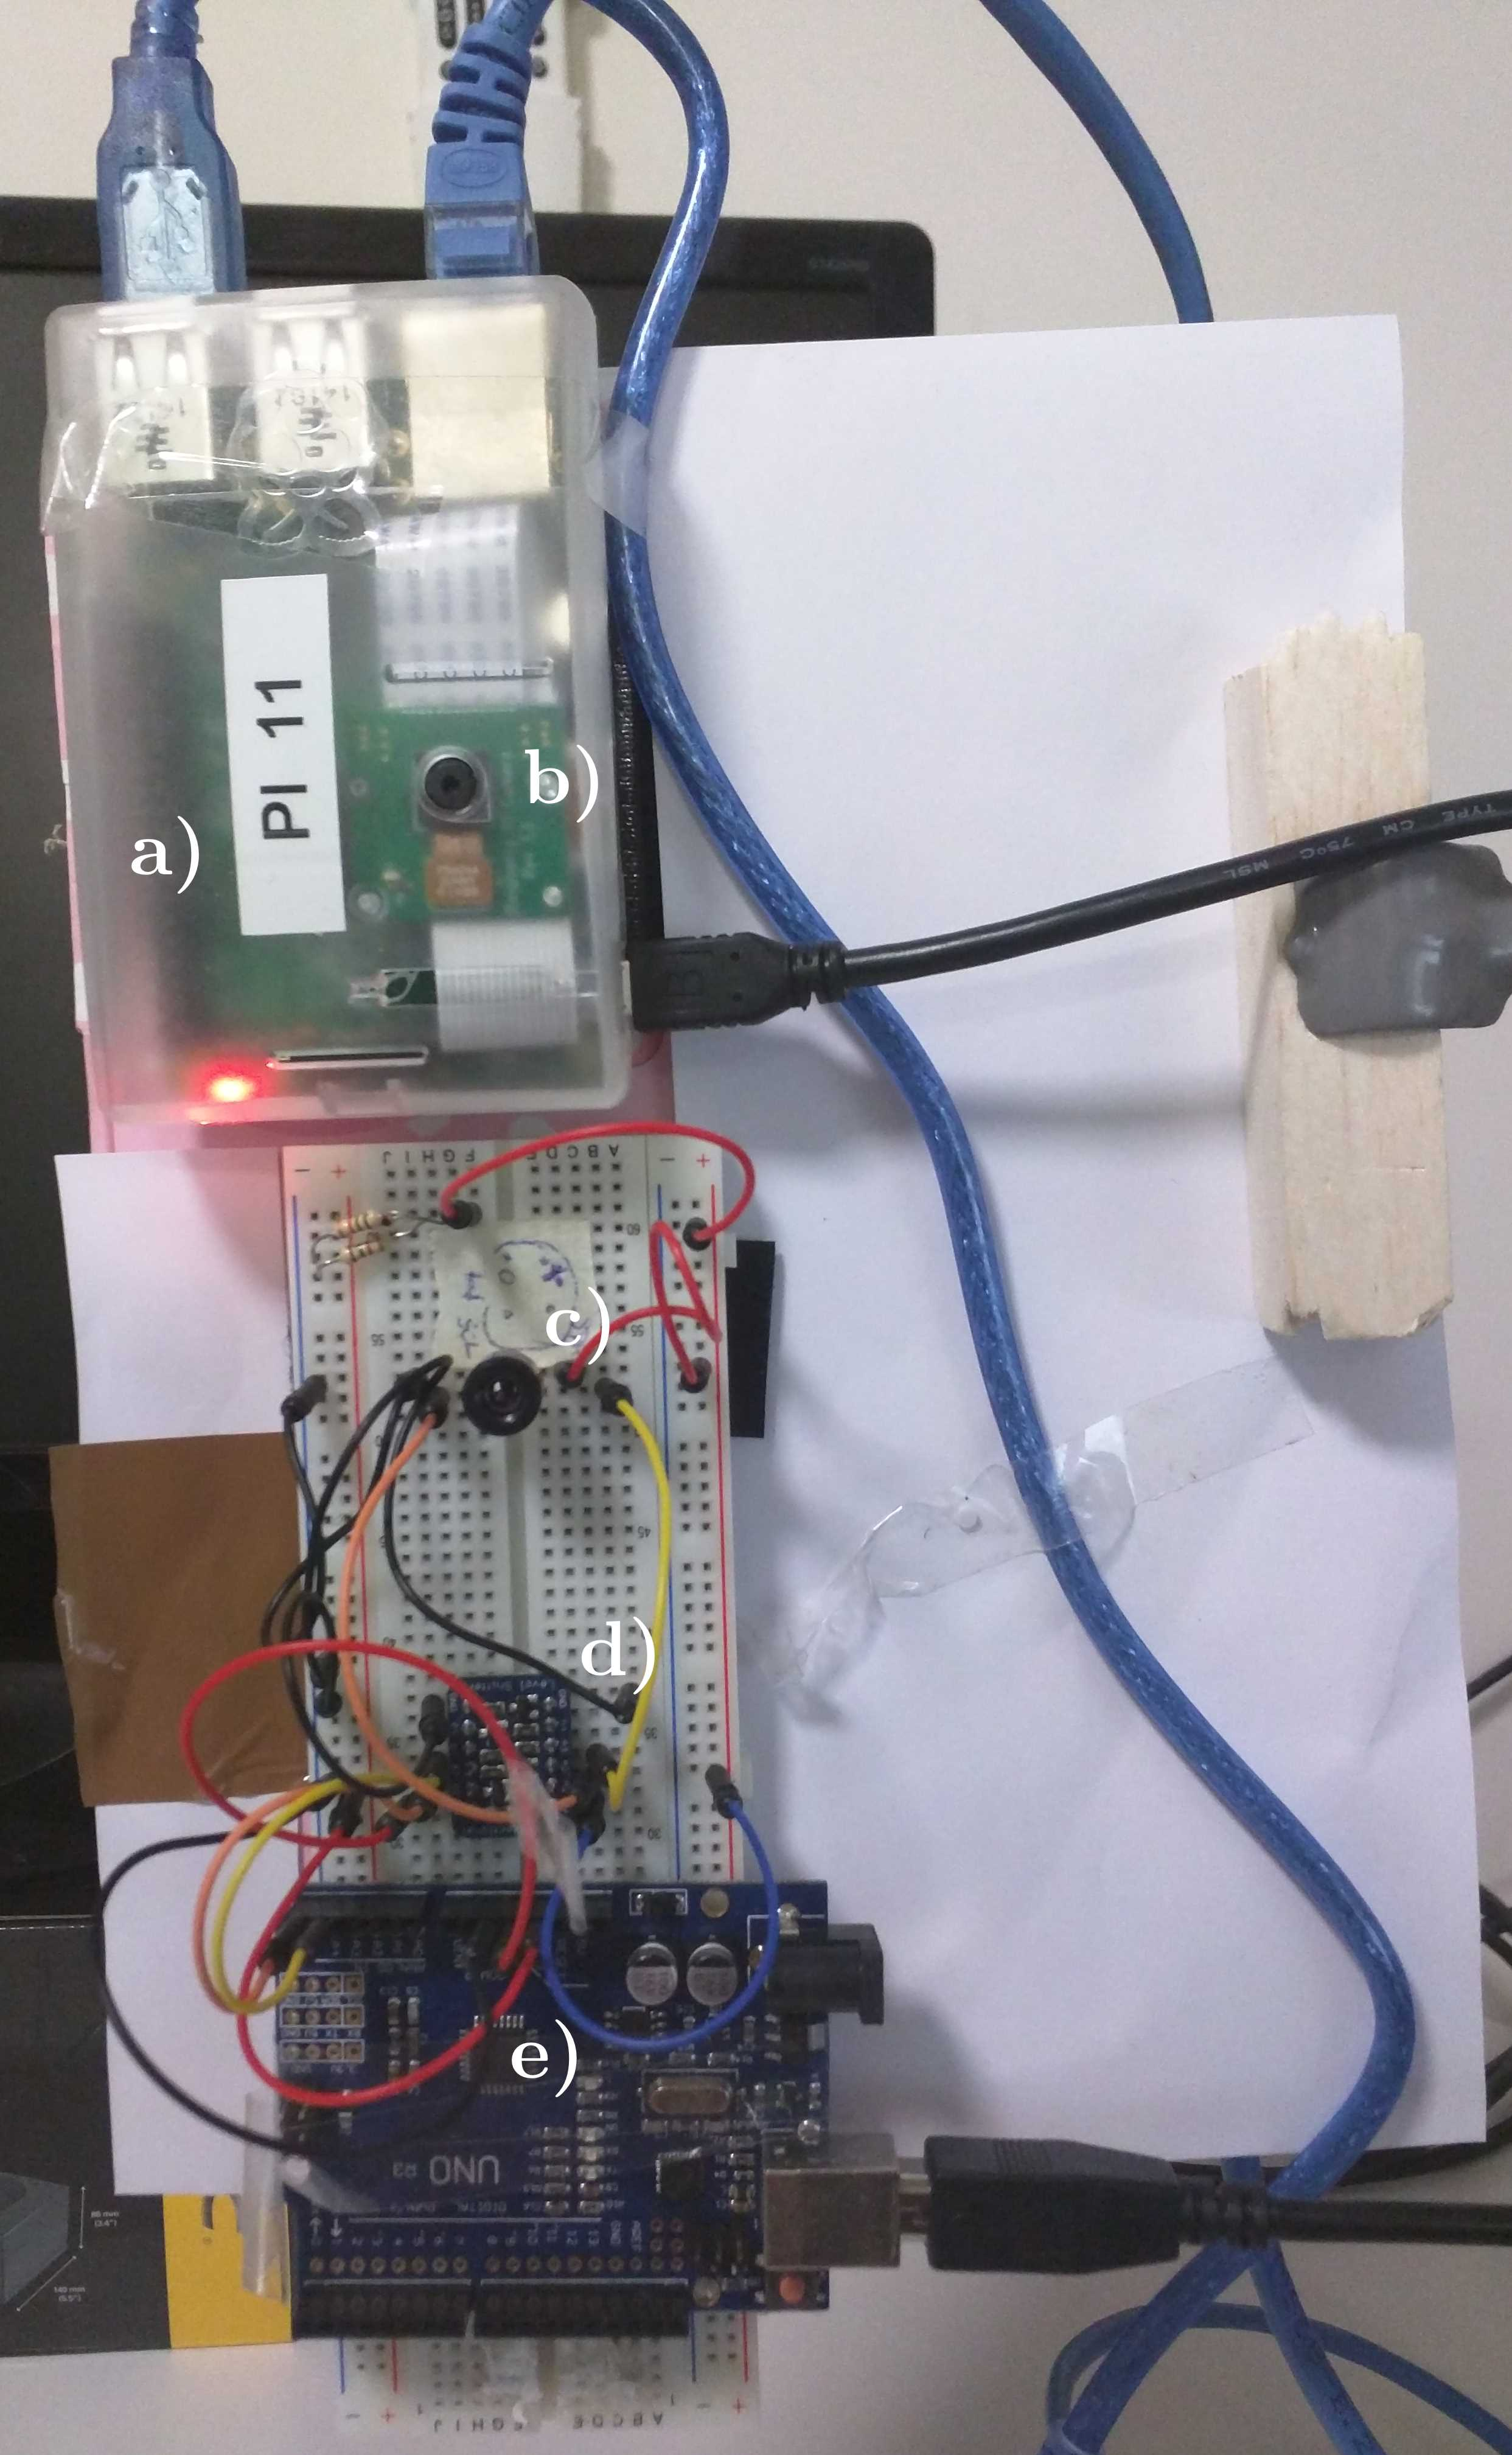
\includegraphics[height=0.7\textheight]{../diagrams/prototypea.jpg}
{\small
\begin{enumerate}[a)]
 \item Raspberry Pi
 \item Camera
 \item \mlx
 \item Level-shifting circuitry
 \item Arduino
\end{enumerate}
}
\caption{Prototype A}
\label{fig:pictures:protoa}
\end{figure}

\begin{figure}
\centering
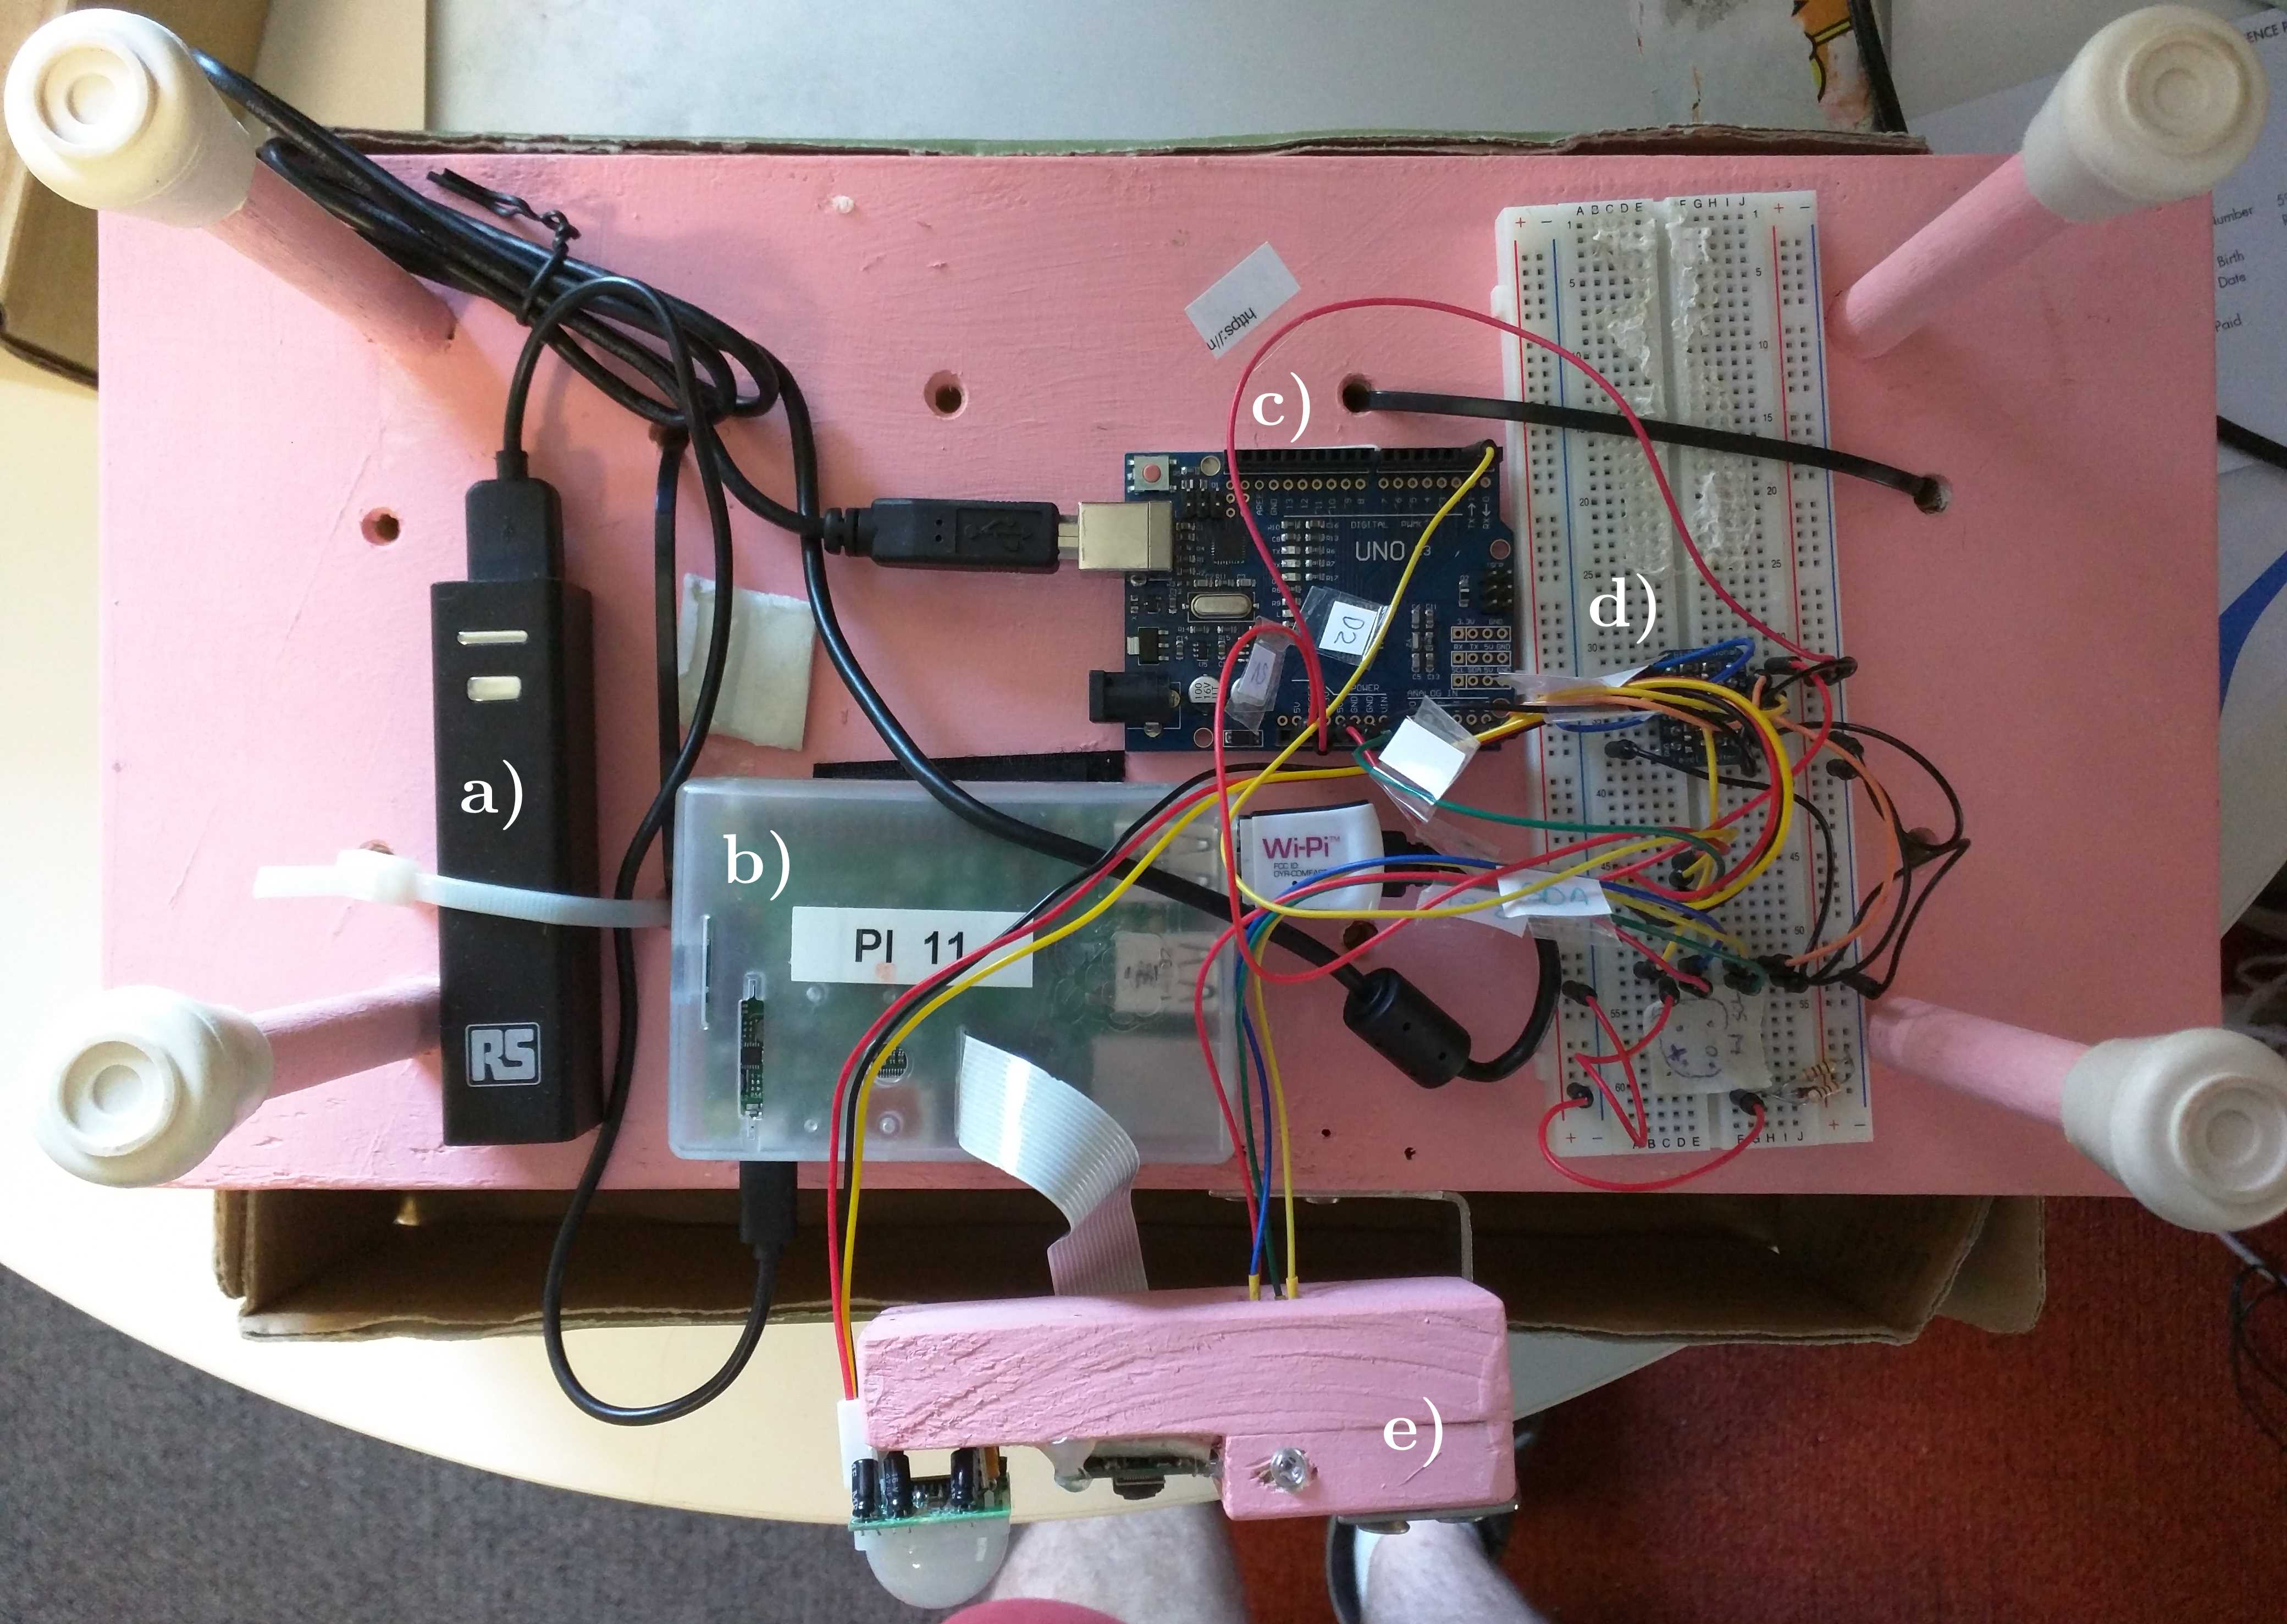
\includegraphics[width=\textwidth]{../diagrams/prototypeb-1.jpg}
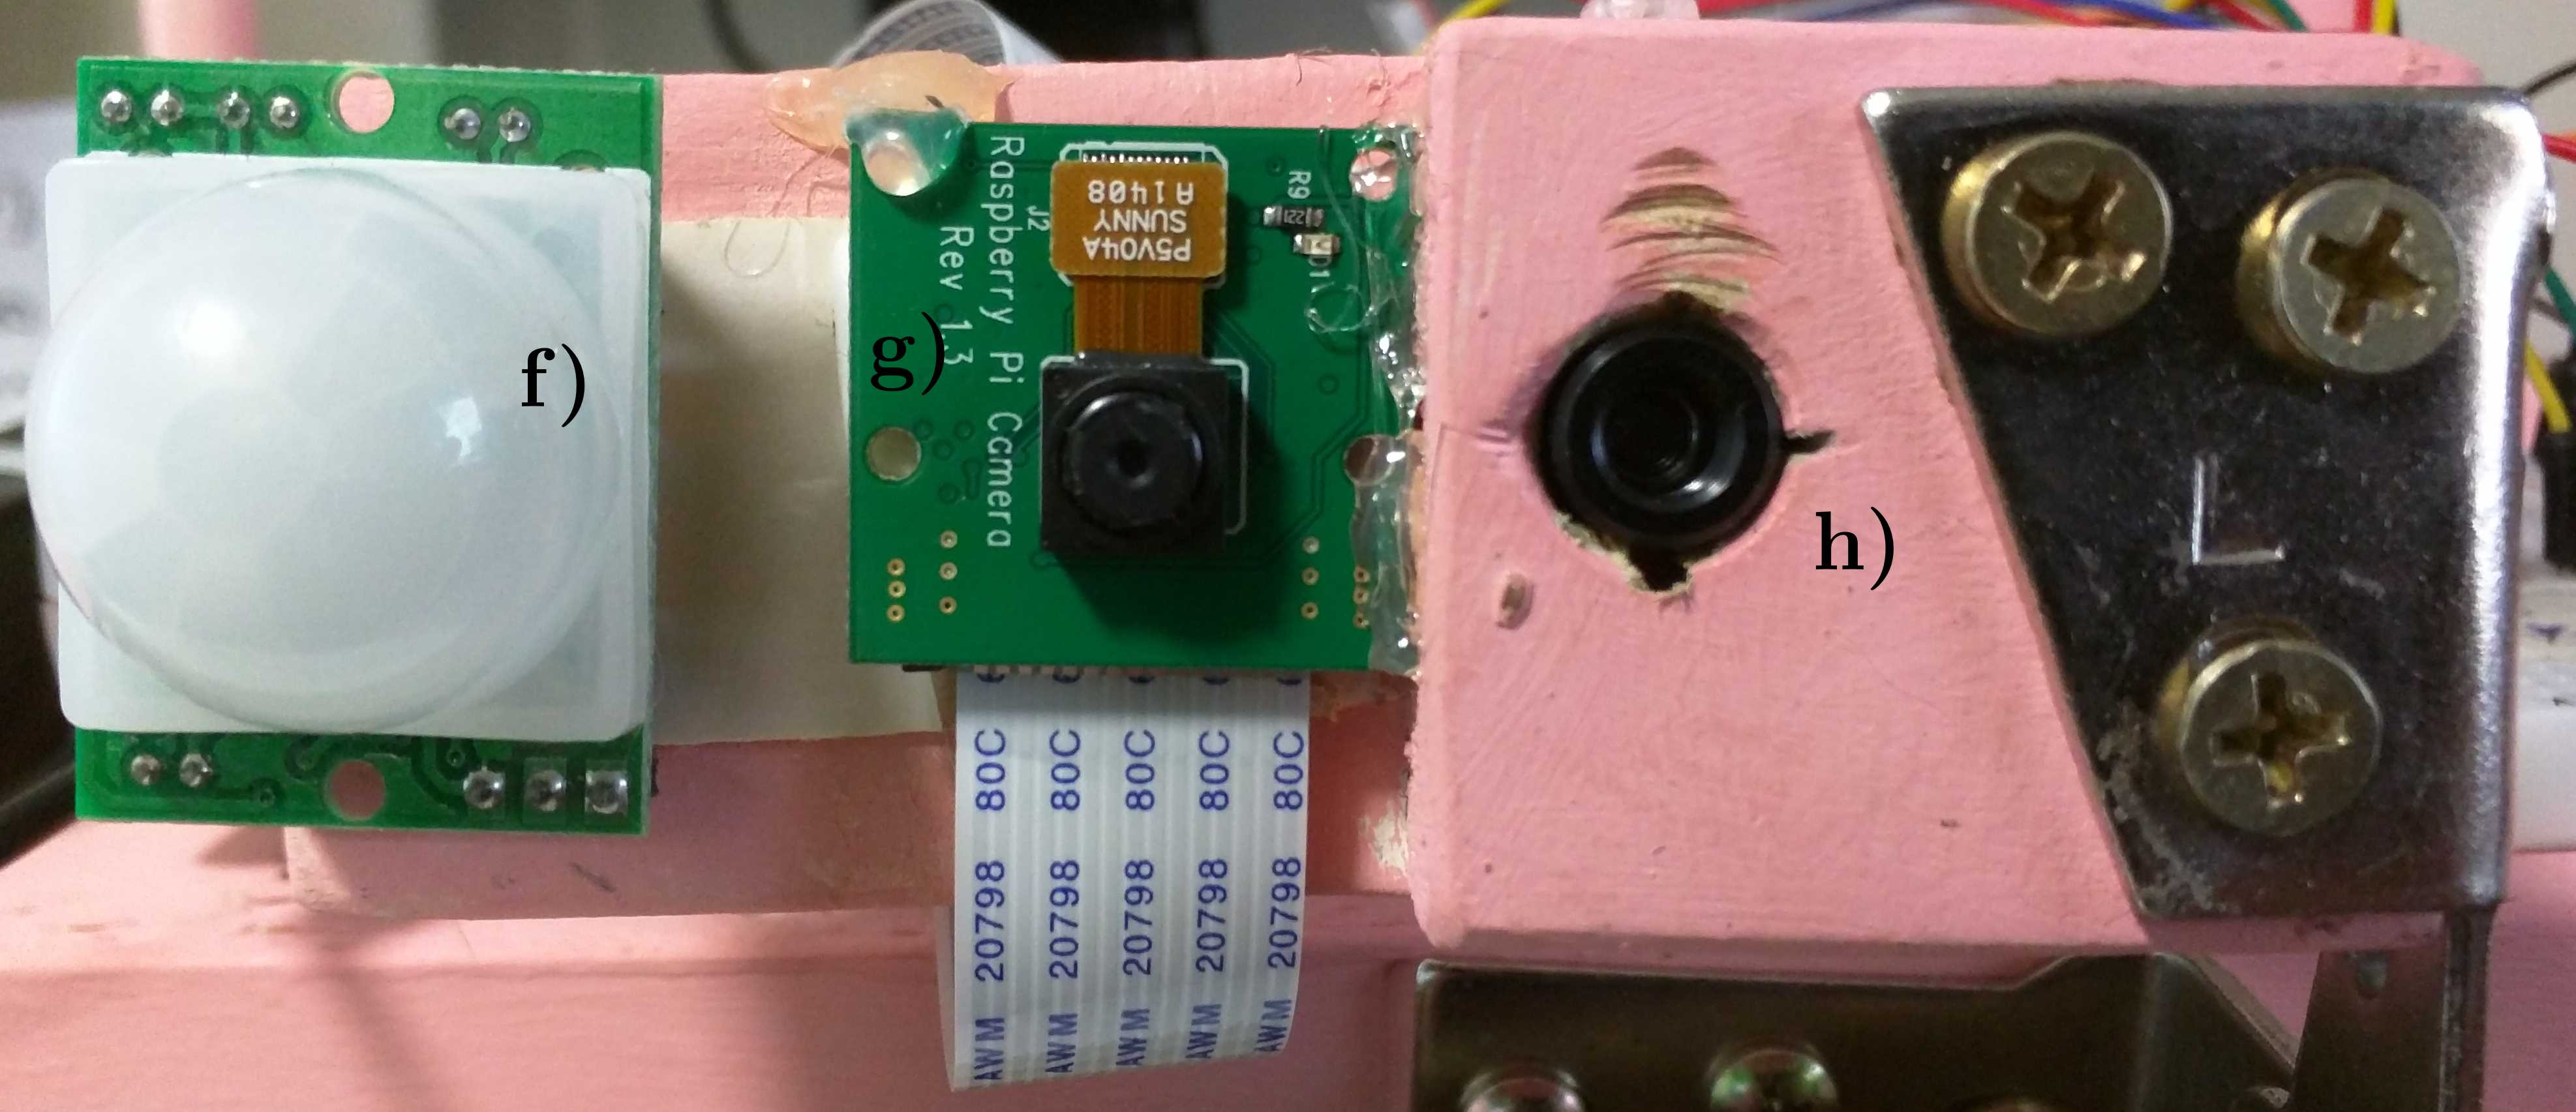
\includegraphics[width=\textwidth]{../diagrams/prototypeb-2.jpg}
{\small
\begin{multicols}{2}
\begin{enumerate}[a)]
 \item Battery pack
 \item Raspberry Pi
 \item Arduino
 \item Level-shifting circuitry
 \item Movable sensor mount
 \item PIR
 \item Camera
 \item \mlx
\end{enumerate}
\end{multicols}
}
\caption{Prototype B}
\label{fig:pictures:protob1}
\end{figure}

\begin{figure}
\centering
\begin{tikzpicture}[node distance=1.7cm]
\node (interwebs) [cbox] {Network};
\node (wifi) [dashbox, left=of interwebs] {\small WiFi / Ethernet};
\node (rpi) [fcont, below=of wifi] {Raspberry Pi \linebreak

  \tikz\node[fbox, minimum width=2.3cm, text width=2.3cm] {\small \ttfamily thinglib};
  \tikz\node[fbox, minimum width=2.3cm, text width=2.3cm] {\small \ttfamily features.py};
};
\node (cam) [box, right=of rpi] {Camera};
\node (usb) [dashbox, below=of rpi] {\small USB Serial};
\node (ard) [fcont, below=of usb] {Arduino \linebreak

  \tikz\node[fbox, minimum width=3.3cm, text width=3.3cm] {\small \ttfamily mlx90620\_driver};
};
\node (iic) [dashbox, left=of ard] {\small \iic};
\node (mlx) [box, below=of iic] {MLX90620};
\node (wire) [dashbox, right=of ard] {\small Interrupt};
\node (pir) [box, below=of wire] {PIR};

\draw [line] (interwebs) -- (wifi);
\draw [line] (wifi) -- (rpi);
\draw [line] (rpi) -- (usb);
\draw [line] (usb) -- (ard);
\draw [line] (ard) -- (iic);
\draw [line] (iic) -- (mlx);
\draw [line] (ard) -- (wire);
\draw [line] (wire) -- (pir);
\draw [line] (rpi) -- (cam);
\end{tikzpicture}
\caption{Prototype B system architecture}
\label{fig:pictures:protob-arch}
\end{figure}
 
 \ifcsdef{mainfile}{}{\bibliography{../references/primary}}
\end{document}
